\begin{figure}
    \centering
    \begin{tikzpicture}[scale=1]
        
        \node at (5,10) {$L$};
        \draw (5,9.5) -- (5,7);
        \draw (5.5,9.5) -- (10,7);
        \node [below] at (5,7) {$E$};
        \node [below right] at (10,7) {\textbf{n}};
        \draw (5,6.5) -- (5,4);
        \draw (5.5,6.5) -- (9,4);
        \draw (4.5,6.5) -- (1,4);
        \node [below] at (5,4) {+};
        \node [below] at (9,4) {$T$};
        \draw (9,3.5) -- (9,1);
        \node [below] at (9,1) {$F$};
        \draw (9,0.5) -- (9,-2);
        \node[below] at (9,-2) {\textbf{digit}};
        \node [below] at (1,4) {$E$};
        \draw (1,3.5) -- (1,1);
        \node [below] at (1,1) {$T$};
        \draw (1,0.5) -- (1,-2);
        \draw (1.5,0.5) -- (5,-2);
        \draw (0.5,0.5) -- (-3,-2);
        \node [below] at (1,-2) {*};
        \node [below] at (5,-2) {$F$};
        \draw (5,-2.5) -- (5,-5);
        \node [below] at (5,-5) {\textbf{digit}};
        \node [below] at (-3,-2) {$T$};
        \draw (-3,-2.5) -- (-3,-5);
        \node [below] at (-3,-5) {$F$};
        \draw (-3,-5.5) -- (-3,-7);
        \node [below] at (-3,-7) {\textbf{digit}};
    \end{tikzpicture}
    \caption{Vector image}
    \label{fig:my_label}
\end{figure}



\begin{figure}[h]
    \centering
    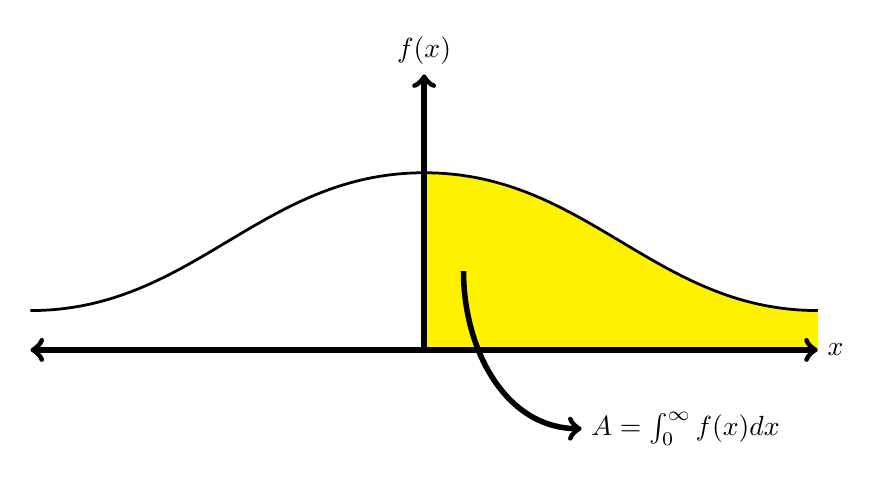
\begin{tikzpicture}[scale=0.5]
        %\draw [ultra thick, help lines] (-10,-10) grid (10,10);
        %\draw [line width=2pt, rounded corners, fill=red] (0,0) rectangle (3,5);
        \path [fill=yellow] (0,4.5) to [out=0,in=180] (10,1) -- (10,0) -- (0,0) -- (0,4.5);
        \draw [line width=2pt, <->] (-10,0) -- (10,0);
        \draw [line width=2pt, <-] (0,7) -- (0,0);
        %\draw [blue, line width=4pt, <->] (0,0) -- (5,5) -- (-5,5) -- (-5,-2);
        %\draw [blue, line width=5pt, fill=blue] (7,7) circle [radius=.1];
        %\draw [red, domain=-4*pi:4*pi, line width=3pt, samples=100] plot (\x,{5*sin(\x r/2)});
        \draw [line width=1pt] (-10,1) to [out=0,in=180] (0,4.5) to [out=0,in=180] (10,1);
        
        \node [above] at (0,7) {$f(x)$};
        \node [right] at (10,0) {$x$};
        
        \draw [->, line width=2pt](1,2) to [in=180, out=-90] (4,-2);
        
        \node [right] at (4,-2) {$A = \int_0^{\infty}f(x) dx$};
        
    \end{tikzpicture}
    \caption{Test}
\end{figure}
